%% The ubcdiss class provides several options:
%%   gpscopy (aka fogscopy)
%%       set parameters to exactly how GPS specifies
%%         * single-sided
%%         * page-numbering starts from title page
%%         * the lists of figures and tables have each entry prefixed
%%           with 'Figure' or 'Table'
%%       This can be tested by `\ifgpscopy ... \else ... \fi'
%%   10pt, 11pt, 12pt
%%       set default font size
%%   oneside, twoside
%%       whether to format for single-sided or double-sided printing
%%   balanced
%%       when double-sided, ensure page content is centred
%%       rather than slightly offset (the default)
%%   singlespacing, onehalfspacing, doublespacing
%%       set default inter-line text spacing; the ubcdiss class
%%       provides \textspacing to revert to this configured spacing
%%   draft
%%       disable more intensive processing, such as including
%%       graphics, etc.
%%

\documentclass[gpscopy,twoside,balanced,onehalfspacing,11pt]{ubcdiss}

\usepackage{mlmodern}
\usepackage[margin=1.25in]{geometry}
\usepackage[numbers]{natbib}
\usepackage{checkend}	% better error messages on left-open environments
\usepackage{booktabs} % nicer tables
\usepackage{graphicx}
\usepackage{imakeidx} \makeindex[intoc]
\usepackage{url} \urlstyle{sf} % should come before hyperref
\usepackage[format=hang,indention=-1cm,labelfont={bf},margin=1em]{caption}
\usepackage{xcolor}
\usepackage{amsmath}
\usepackage{amsthm}
\usepackage{amssymb}
\usepackage{comment}

% https://www.grad.ubc.ca/current-students/dissertation-thesis-preparation/fonts-print
\usepackage[
  bookmarks,bookmarksnumbered,
  pagebackref,linktocpage,
  colorlinks=true,
  linkcolor=blue,
  urlcolor=blue,
  citecolor=blue,
  pdftitle={sszz},
  pdfauthor={Jonathan Chan}
]{hyperref}
\renewcommand*{\backrefalt}[4]{
\textcolor{gray}{\ifcase #1
\or
$\hookrightarrow$ page #2
\else
$\hookrightarrow$ pages #2
\fi}}

% idk if I'll have acronyms as opposed to just an index...
\usepackage[printonlyused,nohyperlinks]{acronym}
\renewcommand{\acsfont}[1]{{\scshape \MakeTextLowercase{#1}}}

% needs to come after hyperref and mathtools
\usepackage[capitalise, noabbrev]{cleveref}

% this fixes the appearance of DOI links in the Bibliography, somehow
\newcommand{\doi}[1]{doi:\href{https://doi.org/#1}{\textsf{#1}}}

% custom style and macros
\usepackage{style}

\title{sszz}
%\subtitle{}

\author{Jonathan Ho\hspace{0.1em}-\hspace{-0.1em}Wing Chan}
\degreetitle{Master of Science}
\institution{The University of British Columbia}
\campus{Vancouver}
\faculty{The Faculty of Graduate and Postdoctoral Studies}
\department{Computer Science}
\submissionmonth{April}
\submissionyear{2022}

\examiningcommittee{William J. Bowman, Computer Science}{Supervisor}
%\examiningcommittee{Ronald Garcia, Computer Science}{Supervisory Committee Member}
%\examiningcommittee{Alexander J. Summers, Computer Science}{Supervisory Committee Member}
\examiningcommittee{Examiner, Department}{Additional Examiner}
\supervisorycommittee{Your Mom, Department}{Supervisory Committee Member}

\begin{document}
\maketitle
\makecommitteepage

%% The following is a directive for TeXShop to indicate the main file
%%!TEX root = diss.tex

\chapter{Abstract}

The abstract:
\begin{itemize}
  \item is a concise and accurate summary of the thesis
  \item should state the problem, the methods of investigation, and the general conclusions
  \item must not exceed 350 words
  \item should contain keywords that will facilitate automated information retrieval
\end{itemize}
\chapter{Lay Summary}

While people communicate to one another by speaking or writing in natural languages,
we communicate with computers via programming languages to tell them to, say, perform a calculation.
Just as what's said or written must be grammatically correct to make any sense,
programs written in these programming languages must be checked to ensure that they behave nicely.
One desirable property of programs can be termination:
we want to be certain that they'll eventually finish running at some point.
It's impossible to devise a check that can always pick out all terminating programs,
but approximate termination checks can be improved upon to accept more and more terminating programs.
The topic of this thesis is using \emph{sized types}, a powerful strategy for termination checking,
in the setting of a programming language for mathematicians to write computer-verified proofs,
and proving that the programs that sized typing accepts will actually terminate.
%% The following is a directive for TeXShop to indicate the main file
%%!TEX root = diss.tex

\chapter{Preface}

The Preface must include a statement indicating the student's contribution to the following:

\begin{itemize}
  \item Identification and design of the research program,
  \item Performance of the various parts of the research, and
  \item Analysis of the research data.
\end{itemize}

Certain additional elements may also be required, as specified below.

\begin{itemize}
  \item If any of the work presented in the thesis has led to any publications or submissions, all of these must be listed in the Preface. Bibliographic details should include the title of the article and the name of the publisher (ONLY if the article has been accepted or published), and the chapter(s) of the thesis in which the associated work is located.
  \item If the work includes publications or material submitted for publication, the statement described above must detail the relative contributions of all collaborators and co-authors (including supervisors and members of the supervisory committee) and state the proportion of research and writing conducted by the student. For further details, see “Including Published Material in a Thesis or Dissertation”.
  \item If the work includes other scholarly artifacts (such as film and other audio, visual, and graphic representations, and application-oriented documents such as policy briefs, curricula, business plans, computer and web tools, pages, and applications, etc.), all of these must be listed in the Preface (with bibliographical information, if applicable).
  \item If ethics approval was required for the research, the Preface must list the Certificate Number(s) of the Ethics Certificate(s) applicable to the project.
\end{itemize}

The content of the Preface must be verified by the student's supervisor, whose endorsement must appear on the final Thesis/Dissertation Approval form.

\tableofcontents
\cleardoublepage

\listoftables
\cleardoublepage

\listoffigures
\cleardoublepage

\chapter{Glossary}

\begin{acronym}[ANOVA]
\acro{CC}{Calculus of Constructions}
\acro{CC(omega)}[CC$^\omega$]{generalized Calculus of Constructions}
\acro{CIC}{Calculus of Inductive Constructions}
\acro{CIC(E)}[CIC$_E$]{extensional Calculus of Constructions}
\acro{pCuIC}{predicative Calculus of Cumulative Inductive Constructions}
\acro{MLTT}{Martin-L\"of Type Theory}
\end{acronym}

\textspacing

\chapter{Acknowledgements}

I'd like to thank the following people for their support throughout the past two years:

\begin{itemize}
  \item William Bowman.
  \item Lily Bryant, for guidance and resources on proving confluence.
  \item Jordy Dickinson, for exposing me to all sorts of niches of type theory and constructive mathematics,
    and for giving an ear to the most out-of-context problems I was working on.
    I hope you're doing well.
  \item Hazel Levine, for making \href{https://types.pl/}{types.pl} a reality (and letting me in on the fun).
  \item The folks on PL Twitter, the TYPES, Coq, Agda, Idris, and Cedille mailing lists and Zulips,
    and the Proof Assistants Stack Exchange for answering my many questions
    and for asking far more interesting ones.
  \item Finally and most importantly, all my other splabmates at the Software Practices Lab
    for making grad school a way better experience than I could have hoped for,
    especially during an ongoing global pandemic.
    To name a few (by increasing order of name length):
    \begin{quote}
    James Yoo\textsuperscript{\href{https://youtu.be/dQw4w9WgXcQ}{0}}, Chris Chen\punctstack{,}\footnote{honourary splabmate}
    Ron Garcia, Adam Geller, Alex Summers, Braxton Hall, Joey Eremondi, Paulette Koronkevich, Felipe Ba\~nados Schwerter,
    \end{quote}
    and many more, especially those who brought treats for the lab.
\end{itemize}

\vfill

This research was supported by the Canada Graduate Scholarships -- Master’s (CGS M) programme.
Cette recherche a \'et\'e financ\'ee par le Programme de bourses d'\'etudes sup\'erieures
du Canada au niveau de la maitrise (BESC M).

\hfill
\chapter{Dedication}

\begin{center}
\textit{Dedicated to the SPL\punctstack{.}}%
\footnote{Special thanks to James Yoo, who took most of these photos.}

\hfill

% TODO: Ask everyone for permission to use
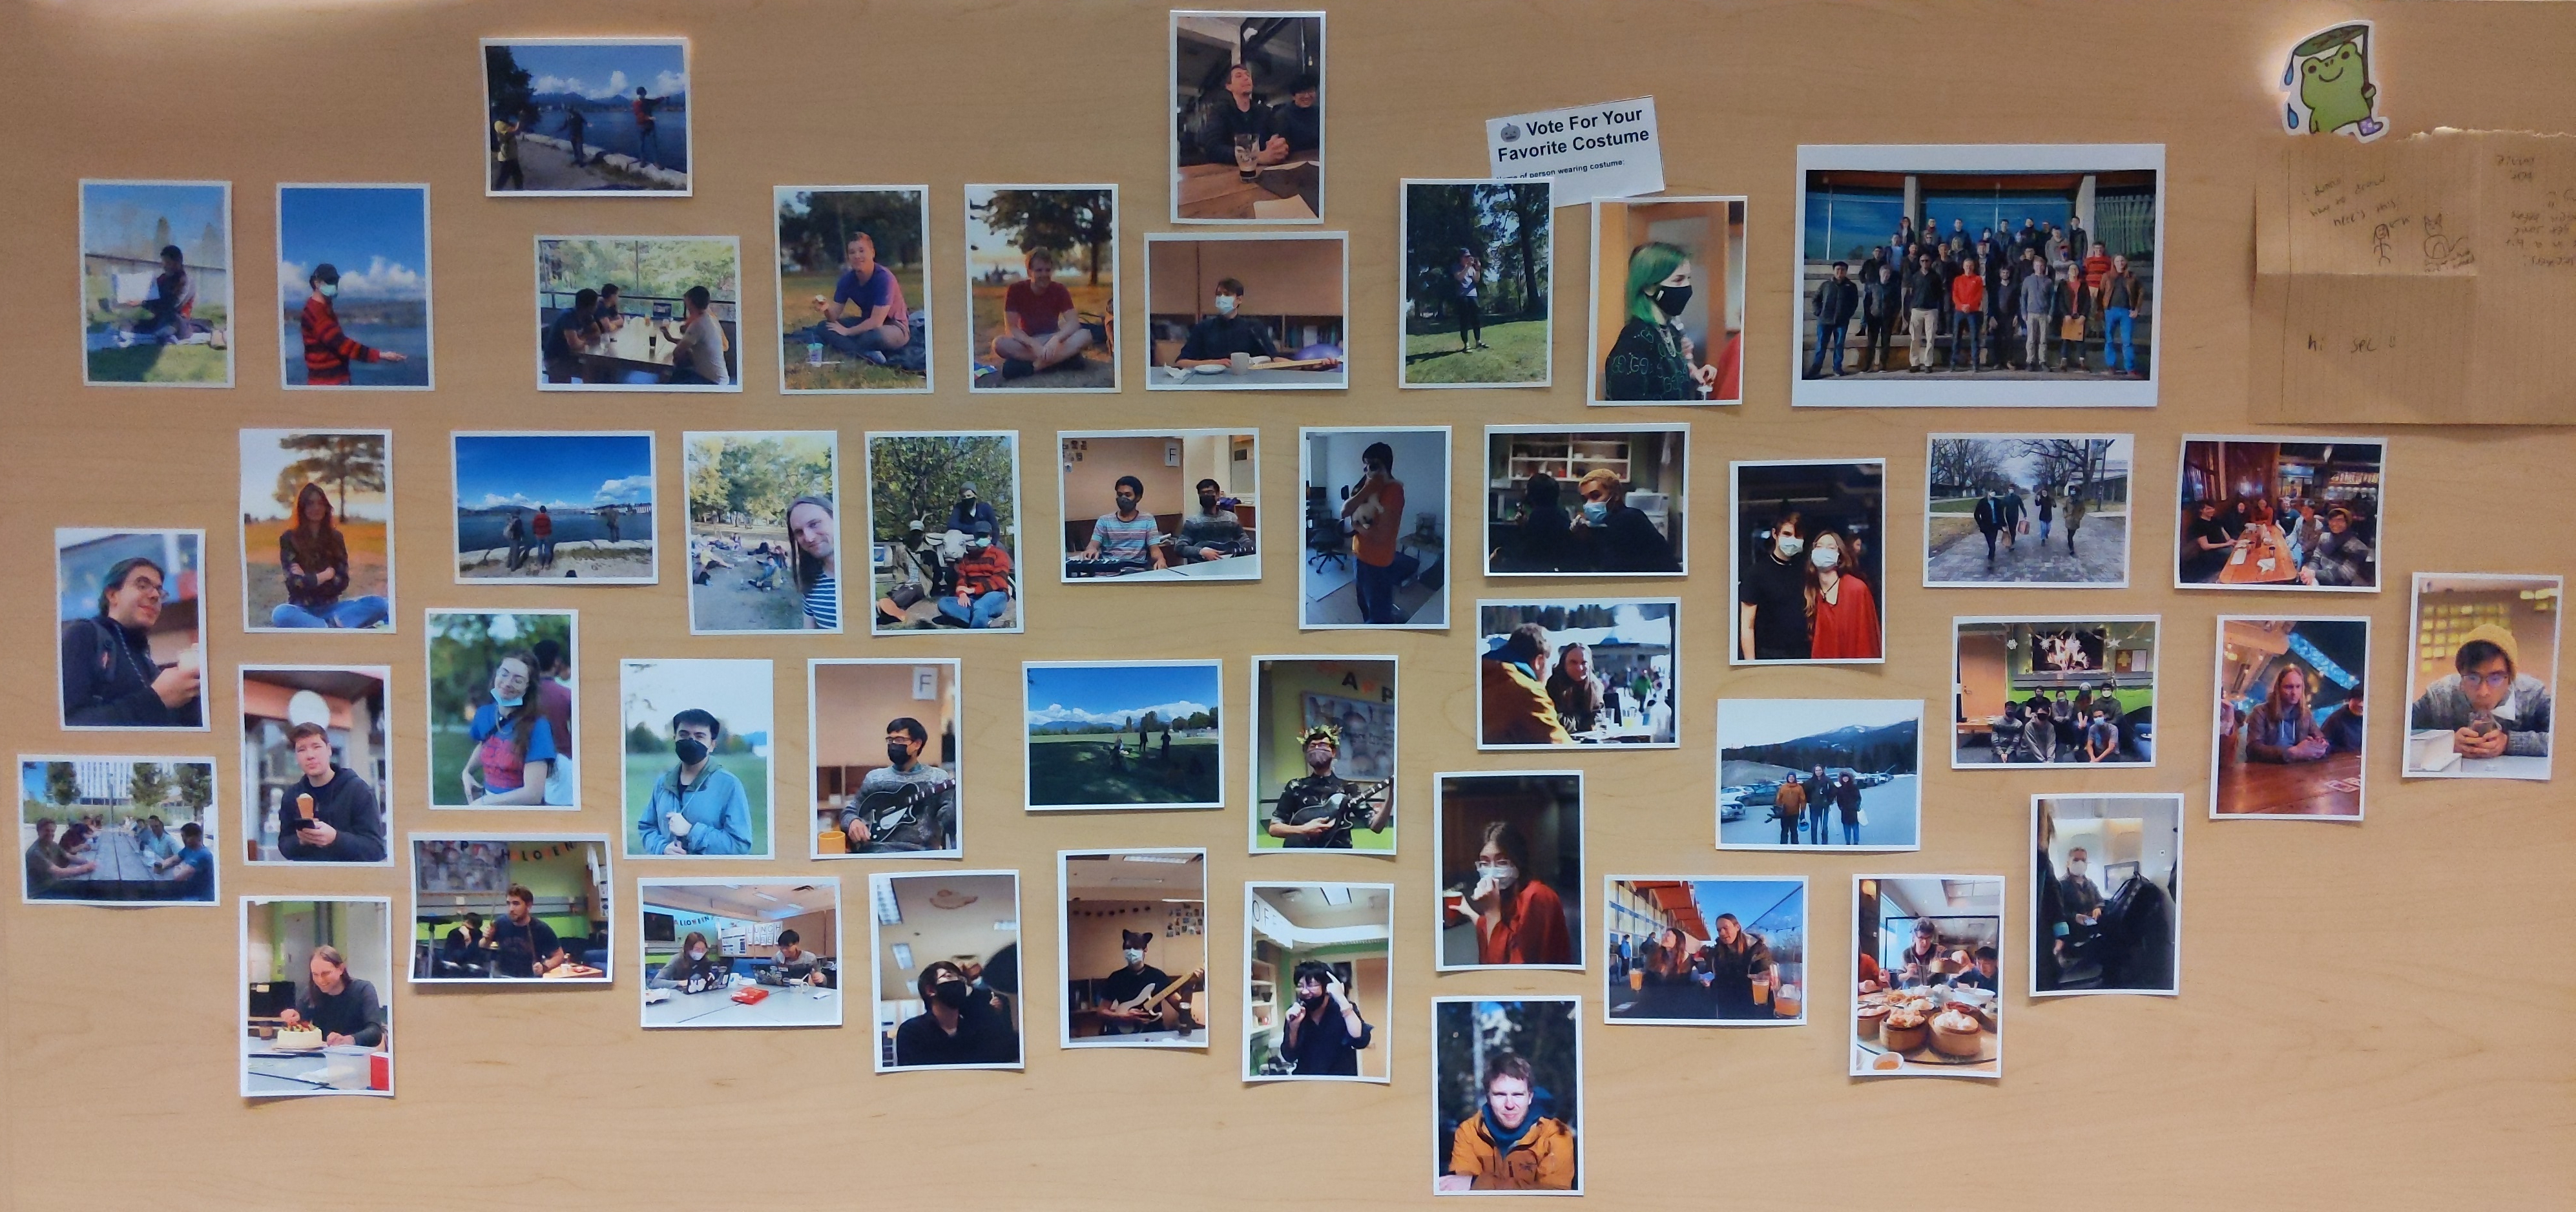
\includegraphics[width=\textwidth]{SPL.jpg}
\end{center}

\mainmatter
\acresetall

\chapter{Introduction} \label{ch:introduction}

A type system is a delicate balance between expressivity and well-behavedness.
More expressivity allows for more programs to be well-typed,
while paradoxically allowing less code to be written,
because some of the onus of ensuring a program is valid is shifted
from the programmer to the process of type checking.
On the other hand, too much expressivity can destroy
desirable metatheoretical properties of the type system ---
strings get be treated as integers, booleans can be called like functions,
and the language falls to chaos and ruin.

The balancing act is particulary perilous for type systems
used by proof assistants for mechanized theorem proving,
because a lack of expressivity can make it too much of a burden to be practically useful,
while it's all to easy to add some convenient, seemingly innocuous feature
that turns out to dismantle the logic of the system,
rendering it unusable for proving.

This thesis deals with dependent type theory, which is commonly used for theorem proving,
together with sized types, a feature for inductively defined types
used to increase the expressivity of recursive functions,
and shows that dependent types can be extended with state-of-the-art sized types
without sacrificing key metatheoretical properties.

\section{Background}

Before we begin, I briefly summarize why dependent types are used for theorem proving,
as well as what sized types have to offer in the context of programming with dependent types.

\subsection{Theorem proving with dependent types} \label{tt}

Many contemporary proof assistants are founded on the Curry--Howard correspondence,
where propositions correspond to types,
proofs of these propositions to terms of those types,
and proof verification to type checking.
Different type theories correspond to different logical systems;
dependent type theories, in particular, correspond to predicate logics.
The primary feature of dependent type theory is the dependent function type,
because it encodes universal quantification by allowing types to \emph{depend on} terms:
the type $\funtype{x}{A}{\app{P}{x}}$ can be interpreted as the statement
``for all objects $x$ in $A$, $P$ holds of $x$'',
with the consequent $\app{P}{x}$ depending on the term $x$.
Other logical constructs can be encoded as well, for example:

\begin{itemize}
  \item Falsehood ($\bot$) as $\funtype{P}{\Prop}{P}$,
    (where $\Prop$ is the type of all propositions),
    the statement that \emph{all} propositions hold;
  \item Implication as $\funtype{\any}{A}{B}$
    (or $\arr*{A}{B}$ for short),
    where $B$ holds only when given a proof of $A$;
  \item Negation as $\arr*{A}{\bot}$,
    or that proving $A$ will yield a falsehood; and
  \item Truthhood as $\funtype{P}{\Prop}{\arr*{P}{P}}$\punctstack{,}%
    \footnote{This encoding is slightly simpler than
    the negation of falsehood $\arr*{\bot}{\bot}$,
    particularly when written out in full.}
    which is trivially inhabited by the identity function
    $\fun{P}{\Prop}{\fun{p}{P}{p}}$;
\end{itemize}
and many other logical connectives such as existential quantification, conjunction, and disjunction.

A key metatheoretical property that a type theory must satisfy
for its interpretation as a logical system to be valid is \emph{consistency}:
falsehood cannot be proven.
In other words, there must not be any term whose type is $\funtype{P}{\Prop}{P}$.
Otherwise, any proposition would be provable,
which goes against the intuition of how a logical system should behave.

The two most important components of a formal description of a dependent type theory
are its typing judgement, whose rules describe when a term has a certain type,
and its equality judgement(s), whose rules describe when two terms are equal.
The latter is relevant in dependent types because they allow determining that,
for instance, a proof of \mbox{$\app{P}{(\app{(\fun{y}{A}{y})}{x})}$}
is in fact also a proof of $\app{P}{x}$.
Naturally, equality is sometimes described in terms of reduction judgements,
governed by the rules of computation.
This means that, in contrast to nondependent type systems,
whether type checking always terminates depends on whether the language is normalizing.
The issue gets even more complicated with more complex forms of reduction like recursion.

\subsection{Recursive programming with sized types} \label{ss}

Inductively defined data and recursive functions on them
are indispensible tools of dependently-typed programming,
allowing the expression of a variety of constructs, programs, and their properties.
A crucial restriction on recursive functions
in proof assistants such as Agda, Coq, Idris, Lean, and more
is that recursive functions must be \emph{guarded by destructors}\index{guardedness}
and only recur on structurally smaller arguments~\citep{guard}.
This guardedness check is statically done before or during type checking and,
to vastly simplify, ensures that recursive calls occur only on syntactic subarguments:
if the original argument is some natural $\app{\succ*}{n}$, then the function recurs only on $n$;
if it's some list $\app{\cons*}{\hd}{\tl}$, then it recurs only on $\tl$;
and so on.

Although this is usually referred to as a syntactic termination check,
and termination is essential in ensuring decidability of type checking,
the key desired property is rather consistency.
Indeed, a type theory may be consistent yet nonnormalizing
(as is the case with an impredicative\index{impredicativity},
definitionally proof-irrelevant $\Prop$ universe~\citep{impred-proof-irrel}),
but unrestricted recursion easily proves an inconsistency:
the recursive function $f$ defined by $\fun{P}{\Prop}{\app{f}{P}}$,
for instance, can be assigned type $\funtype{P}{\Prop}{P}$,
in addition to being nonterminating.

While the guardedness check, being based on the elimination principles of inductive types,
yields terminating functions and a consistent type theory,
it has known disadvantages:

\begin{itemize}
  \item Calling some other function on a subargument prior to a recursive call is disallowed,
    even if that function doesn't change the structure of that subargument,
    because the input of the recursive call is no longer exactly the syntactic subargument.
    For instance, a recursive function on lists cannot first map over the sublist,
    even though the usual mapping function doesn't change the length of a list
    and therefore presents no threat to termination.
  \item Some proof assistants (Coq, for one) will inline functions and even unfold recursive functions
    so that the guardedness check has more information
    and that more recursive functions pass the check.
    However, this too has its disadvantages:
    \begin{itemize}
      \item Programs become nonmodular and noncompositional:
        not only do recursive functions that require inlining
        depend on the implementation of inlined functions,
        they may also depend on their specific implementation details,
        and even a minor syntactic change otherwise equivalent to the original
        can break guardedness~\citep{CIC-hat-minus}.
      \item As aptly summarized by \citet{coqterm},
        \begin{quote}
        \begin{singlespace}
        \textit{{\rm [\ldots]} unfold{\rm [ing]} all the definitions used in the body of the function, do{\rm [ing]} reductions, e.t.c.
        {\rm [\ldots]} makes typechecking extremely slow at times.
        Also, the unfoldings can cause the code to bloat by orders of magnitude and become impossible to debug.}
        \end{singlespace}
        \end{quote}
    \end{itemize}
\end{itemize}

In cases where the guardedness check fails on terminating functions,
the programmer can refactor the function to recur on a different, related argument,
such as the length of a list in the example above,
but this requires additional work and may bloat programs
with extra code solely for satisfying the guardedness check
that detracts from the programs' original intent.
Alternatives to the syntactic guardedness check that avoid these issues are type-based checks,
where the type system itself is augmented so that successful type checking
immediately guarantees termination and consistency.

The one this thesis focuses on is \emph{sized typing}\punctstack{,}%
\footnote{The other common one uses \emph{guarded types}~\citep{guarded-types}.}
where inductive types are annotated with size information,
and constructors construct constructions whose size is larger than that of their subarguments.
In short, the notion of a ``smaller'' subargument is encoded within the types,
no longer requiring syntactic analysis to determine.
Finally, a recursive function is well typed only if it recurs on an argument
whose size is smaller than that of the original argument.

Because well-typedness is the only required condition,
calling some other function before a recursive call is allowed
as long as that function is \emph{size preserving}\index{size preservation}.
For the list mapping example above,
this means that if the sublist of elements of type $\tau$ has size $s$,
then the mapping function must have type $\arr*{\List{\tau}{s}}{\List{\tau}{s}}$.
Notice that the implementation of the mapping function isn't required,
merely its type, thereby avoiding the issues with inlining and unfolding.

This thesis then introduces Sizey \textsc{mc}Type Theory (\lang),
a sized dependent type theory that I prove to be logically consistent consistent
and therefore suitable for both recursive programming and theorem proving.

\section{Overview}

But what need is there for yet another sized type system?
Since \citet{hughes}, there has been a little over two decades' worth of past work on sized types.
\citet{flationary} notes that it has been the topic of at least five dissertations.
This chapter alone names a dozen different type systems with sized types.
There have been many advancements along the way,
but none quite satisfactory to close the matter,
especially when it comes to dependent types.

\lang and this thesis as a whole does not aim to resolve
all of the remaining problems of sized types left open by these past works.
Instead, the purpose is threefold:

\begin{itemize}
  \item To fill an existing gap in sized dependent type theories.
    Two modern sized type features are higher-rank and bounded size quantification,
    and there exist a few dependent type theories with one or the other,
    but not both, to my knowledge.
    On the other hand, they are currently in Agda's implementation of sized types.
    By proving the consistency of \lang, a novel type theory with these two features,
    I bring the theoretical state-of-the-art closer to practice. \\
  \item To demonstrate the viability of using a syntactic model to prove consistency
    of a sized type theory.
    Doing so from scratch through a set-theoretic model is notoriously difficult,
    and often requires sacrifices to and constraints on the type theory;
    see Sacchini's dissertation~\citep{CIC-hat-minus} or \CIChatstar~\citep{CIC-hat-star},
    for instance.
    Instead, a syntactic model relies on the consistency of the language in which I'm modelling,
    and requires no additional deep mathematical knowledge.
  \item To reopen the discussion on sized dependent types.
    Since the discovery of the inconsistency of Agda's sized types~\citep{infinity},
    progress appears to have stagnated a little.
    In later chapters, I examine these difficulties as they might apply to \lang
    and its interpretation in the syntactic model.
\end{itemize}

In this section I describe and justify the design of
the dependent types and the sized types of \lang,
explain how a syntactic model is used to prove its consistency,
and briefly outline the structure of the proof.

\subsection{Dependent types}

As a simple but expressive foundation for dependent types,
I start with the Generalized Calculus of Constructions (\GCC)\index{Calculus of Constructions!Generalized \textasciitilde} \citep{GCC-Coquand},
which has the following features:

\begin{itemize}
  \item \textbf{Dependent function types}, as is standard in the Calculus of Constructions (CC)~\citep{CoC}\index{Calculus of Constructions};
  \item \textbf{Definitions}, \ie locally-named expressions;
  \item \textbf{Universes \ala Russell}\index{universes \ala Russell}, where the types of types are themselves terms
    (as opposed to universes \ala Tarski\index{universes \ala Tarski}, where their \emph{encodings} are terms);
  \item An \textbf{impredicative universe}\index{impredicativity} $\Prop$ such that function types into types in $\Prop$
    are themselves in $\Prop$;
  \item A \textbf{cumulative hierarchy of universes}\index{cumulativity} such that $\Type{i}: \Type{i+1}$,
    any term in $\Type{i}$ is also in $\Type{j}$ given \emph{universe levels}\index{universe level} $i \leq j$,
    and there is a subtyping relation\index{subtyping} on types induced by this inclusion; and
  \item \textbf{Untyped definitional equality} stating when two terms are judgementally equal to one another.
\end{itemize}

These features cover many modern proof assistants.
To name a few, in terms of universes,
Coq and Arend have all of the above;
Lean lacks cumulativity; and
Agda and \Fstar lack cumulativity and an impredicative universe.
On the other hand, these proof assistants all have some form of
\emph{universe level polymorphism},
but this is much more complex and largely orthogonal to sized types
and the syntactic model.

Perhaps the most contentious design decision so far is the use of untyped equality,
as can be found in Coq, over typed equality, as can be found in Agda.%
While typed equality is considered to ``have clearer mathematical semantics''~\citep{typed-NbE},
its judgement depends on the typing judgement;
meanwhile, since types can depend on terms,
typing itself depends on equality to check whether one type can be used in place of another.
As we'll see in \cref{sec:syntactic-model}, these mutually-defined judgements would greatly complicate the proofs,
so I settle for untyped equality instead.

On top of \GCC, I add two inductive definitions featured in Martin--L\"of type theory (MLTT)~\citep{mltt}\index{Martin--L\"of type theory}:
the \emph{Peano naturals} and \emph{well-founded trees}\punctstack{,}%
\footnote{The types of well-founded trees are also known as \emph{W types}.}
augmented with sizes.
As the simplest nontrivial inductive,
the naturals make it easy to demonstrate intuitive uses of sized inductives.
On the other hand, well-founded trees are an example of \emph{generalized} inductives,
with recursive arguments that are functions that return well-founded trees.
They can encode all (nonnested) inductives,
as well as their induction principles \citep{whynotW} if there are dependent pair types
and a \emph{propositional equality}\index{propositional equality} type.
I don't add inductive types in general in their place
because the syntactic baggage that comes with handling the generalization
obscures the intuition behind sized inductive types and the syntactic model,
while it's easy to see how one \emph{could} go from the naturals and well-founded trees
to inductive types in general.

\subsection{Sized types}\label{sec:sized-types}

Sized types are introduced with explicit size quantification $\Funtype{\alpha}{\tau}$,
size abstraction $\Fun{\alpha}{e}$, and size application $\App{e}{s}$.
Sizes themselves consist of size variables as well as a \emph{base size}
and a \emph{size successor operator}.
This is the standard for size expressions in sized type systems.
Some augment the size grammar with addition of or scalar multiplication of size variables,
for instance, increasing expressivity at the expense of complexity.
To keep things simple, I don't include these features and stick to successor sizes.
Note that size expressions here are \emph{not} terms,
and their quantifications, abstractions, and applications
are syntactically distinct from those of terms,
similar to how, in nondependent polymorphic type systems,
types are distinct from terms.

Having explicit sizes differs from some most prior sized type systems where,
extending the type polymorphism analogy,
there is only implicit \emph{rank-1} or
\emph{prenex} size quantification:
size quantifications never appear inside of a type,
and in fact all size abstractions and applications are fully inferred.
Explicit sizes, in contrast, let us express
\emph{higher-rank} size quantification,
which allow for more expressiveness:
for instance, supposing we have cons lists parametrized over some sized type $\tau$,
one could write a size-preserving mapping function over a list
that leaves the sizes untouched.
The type of such a function might be

\vspace{-0.25\baselineskip}
$$\Funtype{\alpha}{\arr*{(\Funtype{\beta}{\arr*{\App{\tau}{\beta}}{\App{\tau}{\beta}}})}{\app{\List*}{(\App{\tau}{\alpha})}}{\app{\List*}{(\App{\tau}{\alpha})}}}.$$

Along with higher-rank sizes, I also include \emph{bounded} size quantification $\Funtype<{\alpha}{s}{\tau}$
and abstraction $\Fun<{\alpha}{s}{e}$.
An order on sizes is induced by these bound instantiations and the successor operator;
this order has nothing to do with subtyping,
and in particular we do \emph{not} have subtyping relations between
$\N{\alpha}$ and $\N{\sss{\alpha}}$, for instance.
Fixpoint expressions recur on smaller sizes according to the order,
summarized by the below typing rule.
%
\begin{mathpar}
\inferrule[]{
  \check{\Phi, \alpha; \Gamma, f: \Funtype<{\beta}{\alpha}{\subst{\tau}{\alpha}{\beta}}}{e}{\tau}
}{
  \infer{\Phi; \Gamma}{\fix{f}{\alpha}{\tau}{e}}{\Funtype{\alpha}{\tau}}
}
\end{mathpar}

Bounded sizes were originally introduced to avoid complex
\emph{semi-continuity} or approximative \emph{polarity}
requirements on fixpoints' types in the presence of an \emph{infinite size}\index{infinite size}
that is strictly larger than all sizes.
Although I don't include an infinite size,
this style of recursion is more elegant because it corresponds neatly to well-founded induction on sizes.

In summary, the sized type features I include are:

\begin{itemize}[noitemsep]
  \item \textbf{Explicit size} quantification $\Funtype{\alpha}{\tau}$,
    abstraction $\Fun{\alpha}{e}$, and
    application $\App{e}{s}$;
  \item A \textbf{simple size grammar} with size variables $\alpha$, a base size $\circ$, and successors $\sss{s}$;
  \item \textbf{Higher-rank sizes}, \eg $\arr*{(\Funtype{\alpha}{\tau})}{\sigma}$;
  \item \textbf{Bounded size} quantification $\Funtype<{\alpha}{s}{\tau}$ and
  abstraction $\Fun<{\alpha}{s}{e}$.
\end{itemize}

Notably, these are all features found in Agda's implementation of sized types.
The only missing feature is the infinite size,
since its properties and its use are known to be inconsistent in Agda.
A demonstration of the inconsistency of a hypothetical infinite size in \lang
is given in \cref{sec:infinity}.

\subsection{Syntactic model}\label{sec:syntactic-model}

To show that \lang is consistent and therefore a suitable type theory for proofs,
I define for it a \emph{syntactic model}\index{syntactic model}~\citep{syntactic-models}.
This involves defining a translation from \lang into some target type theory
in whose consistency we have more confidence---in this case,
the \emph{Extensional Calculus of Inductive Constructions}\index{Calculus of Inductive Constructions!Extensional \textasciitilde}
(\CICE)~\citep{CICE}.
It, too, has a cumulative hierarchy of universes \ala Russell and an impredicative universe,
augmented with inductive types and \emph{equality reflection}\index{equality reflection},
where a definitional equality between terms can be derived from a propositional one between them.
The most notable difference from \lang, aside from these features and sized types,
is that \CICE uses a typed, declarative equality rather than an untyped, algorithmic equality
to better accomodate equality reflection.
For concision and to avoid confusion, I henceforth refer to the former as \emph{equivalence}\index{equivalence},
and to the latter as \emph{conversion}\index{conversion}.

This translation from \lang to \CICE must be \emph{type preserving}\index{type preservation}%
\footnote{This terminology comes from compilation;
in the context of syntactic modelling, this is rather unhelpfully known as \emph{soundness}.}:
if some term $e$ is well typed under some environments $\Phi; \Gamma$ with some type $\tau$,
then the translated term $\compile{e}$ must also be well typed
under the translated environment $\compile{\Phi}\compile{\Gamma}$
with the translated type $\compile{\tau}$.
By the consistency of \CICE and a type-preserving translation to it,
we prove the consistency of \lang.

\begin{postulate}[Consistency of \CICE]\label{fact:consistency-cice}
There exists no term $\eT$ such that
\mbox{$\type{\mt}{\eT}{\funtypeT{\PT}{\PropT}{\PT}}$}.
\end{postulate}

\begin{theorem}[Consistency of \lang]\label{thm:overview:consistency}
Suppose $\compile{\bot} = \funtypeT{\PT}{\PropT}{\PT}$.
Then there exists no term $e$ such that \mbox{$\type{\mt \mathbin{;} \mt}{e}{\bot}$}.
\end{theorem}
\begin{proof}
Suppose that there were such a term $e$.
By the type-preserving translation, we would have that
$\type{\mt}{\compile{e}}{\funtypeT{\PT}{\PropT}{\PT}}$ holds.
However, this contradicts \cref{fact:consistency-cice},
so there must not be such a term.
\end{proof}

What remains, then, is to define $\bot$ and an appropriate translation from \lang to \CICE
such that $\compile{\bot} = \funtypeT{\PT}{\PropT}{\PT}$,
and to show that this translation is type preserving.
I define my translation by induction on the typing derivations of \lang
rather than merely over its syntax,
ensuring that only well-typed terms have a translation.

Type preservation of the translation is proven by induction on not only the typing derivations,
but also the derivations of the judgements on which the typing rules depend.
In particular, typing depends on subtyping\index{subtyping}, which in turn depends
on \emph{$\alpha$-cumulativity}\index{$\alpha$-cumulativity}~\citep{MetaCoq}
and on the reflexive, transitive, congruent closure of reduction.
Finally, this closure of reduction depends on the reduction rules,
most of which are defined by substitution.
Below are the relevant rules showing these dependencies and an example reduction rule.
%
\begin{mathpar}
\inferrule[]{
  \dots \\\\
  \infer{\Phi; \Gamma}{e}{\sigma} \\\\
  \subtype{\Phi; \Gamma}{\sigma}{\tau}
}{
  \check{\Phi; \Gamma}{e}{\tau}
}

\inferrule[]{
  \acum{\sigma_1}{\sigma_2} \\\\
  \red*{\Phi; \Gamma}{\tau_1}{\sigma_1} \\\\
  \red*{\Phi; \Gamma}{\tau_2}{\sigma_2}
}{
  \subtype{\Phi; \Gamma}{\tau_1}{\tau_2}
}

\inferrule[]{
  \red{\Phi; \Gamma}{e_1}{e_2}
}{
  \red*{\Phi; \Gamma}{e_1}{e_2}
}

\inferrule[]{~}{
  \red{\Phi; \Gamma}{\app{(\fun{x}{\tau}{e})}{e'}}{\subst{e}{x}{e'}}
}
\end{mathpar}

We therefore need some lemmas showing that the translation respects
substitution, reduction, the closure of reduction, $\alpha$-cumulativity, and subtyping
in order to prove type preservation.
In short, substitution satisfies a \emph{compositionality}\index{compositionality} principle,
reduction of terms are equivalent by the \CICE equivalence judgement
$\defeq{\GammaT}{\eT_1}{\eT_2}{\tauT}$,
and $\alpha$-cumulative terms and subtypes are correspondingly \CICE subtypes.
I summarize them here, omitting some hypotheses and sublemmas,
to outline the proof architecture,
which roughly follows the structure of type-preserving compilation by~\citet{wjb}.

\begin{lemma}[Compositionality]\label{lem:overview:compositionality}\hfill
\begin{enumerate}[noitemsep]
  \item $\compile{\subst{e}{x}{e'}} = \subst{\compile{e}}{x}{\compile{e'}}$.
  \item $\compile{\subst{e}{\alpha}{s}} = \subst{\compile{e}}{\alpha}{\compile{s}}$
\end{enumerate}
\end{lemma}

\begin{proof}
By induction on the derivation of $\type{\Phi; \Gamma}{e}{\tau}$.
\end{proof}

\begin{lemma}[Preservation of reduction]\label{lem:overview:pres-red}
If $\red{\Phi; \Gamma}{e}{e'}$ and
$\type{\compile{\Phi}\compile{\Gamma}}{\compile{e}}{\tauT}$
then $\defeq{\compile{\Phi}\compile{\Gamma}}{\compile{e}}{\compile{e'}}{\tauT}$.
\end{lemma}

\begin{proof}
By cases on the derivation of $\red{\Phi; \Gamma}{e}{e'}$,
using inversion on the derivation of $\type{\compile{\Phi}\compile{\Gamma}}{\compile{e}}{\compile{\tau}}$,
\cref{lem:overview:compositionality},
and an application of equality reflection in the case for reduction of fixpoints.
\end{proof}

\begin{lemma}[Preservation of reflexive, transitive, congruent closure of reduction]\label{lem:overview:pres-red*}
If $\red*{\Phi; \Gamma}{e}{e'}$ and
$\type{\compile{\Phi}\compile{\Gamma}}{\compile{e}}{\tauT}$
then $\defeq{\compile{\Phi}\compile{\Gamma}}{\compile{e}}{\compile{e'}}{\tauT}$.
\end{lemma}

\begin{proof}
By induction on the derivation of $\red*{\Phi; \Gamma}{e}{e'}$,
using \cref{lem:overview:pres-red},
subject reduction of \lang,
and subject equivalence of \CICE.
\end{proof}

\begin{lemma}[Preservation of $\alpha$-cumulativity]\label{lem:overview:pres-acum}
If $\acum{\tau_1}{\tau_2}$ and
$\type{\compile{\Phi}\compile{\Gamma}}{\compile{\tau_i}}{\UT_i}$
then $\subtype{\compile{\Phi}\compile{\Gamma}}{\compile{\tau_1}}{\compile{\tau_2}}$.
\end{lemma}

\begin{proof}
By induction on the derivation of $\acum{\tau_1}{\tau_2}$,
using inversion on the derivations of $\type{\Phi; \Gamma}{\tau_i}{U_i}$ and
$\type{\compile{\Phi}\compile{\Gamma}}{\compile{\tau_i}}{\UT_i}$.
\end{proof}

\begin{lemma}[Preservation of subtyping]\label{lem:overview:pres-subtyping}
If $\subtype{\Phi; \Gamma}{\tau_1}{\tau_2}$
and $\type{\compile{\Phi}\compile{\Gamma}}{\compile{\tau_i}}{\compile{U}}$
then $\subtype{\compile{\Phi}\compile{\Gamma}}{\compile{\tau_1}}{\compile{\tau_2}}$.
\end{lemma}

\begin{proof}
By cases on the derivation of $\subtype{\Phi; \Gamma}{\tau_1}{\tau_2}$,
using \cref{lem:overview:pres-red*}, \cref{lem:overview:pres-acum},
subject reduction of \lang,
and subject equivalence of \CICE.
\end{proof}

\begin{theorem}[Type preservation]\label{lem:overview:pres-typing}\hfill
\begin{enumerate}[noitemsep]
  \item If $\wf{\Phi}{\Gamma}$ then $\wf{}{\compile{\Phi}\compile{\Gamma}}$.
  \item If $\type{\Phi; \Gamma}{e}{\tau}$ then $\type{\compile{\Phi}\compile{\Gamma}}{\compile{e}}{\compile{\tau}}$.
\end{enumerate}
\end{theorem}

\begin{proof}
By mutual induction on the derivations of $\wf{\Phi}{\Gamma}$ and $\type{\Phi; \Gamma}{e}{\tau}$,
using \cref{lem:overview:pres-subtyping}.
\end{proof}

The most important properties required of \lang are subject reduction\index{subject reduction},
used in \cref{lem:overview:pres-subtyping},
and confluence\index{confluence}, which is used to show that subtyping is transitive,
which in turn is used to prove the inversion principles for the typing judgement.

This proof structure is possible by virtue of the non-mutuality of the judgements of \lang
due to the use of untyped conversion\index{conversion} (and hence untyped reduction).
If it were instead typed, then it would mutually depend on typing and subtyping as well,
and the above lemmas would circularly depend on one another~\citep{wjb}. \\

\section{Related Work}

The history and development of sized types spans over two decades of past work,
and that of dependent types far more than that.
I therefore mention here only past work that are directly relevant
or that I refer to again in later chapters.

\subsection{Dependent type theories}

\GCC\index{Calculus of Constructions!Generalized \textasciitilde}
was originally proposed by \citet{GCC-Coquand},
adding a universe hierarchy to CC\index{Calculus of Constructions} with untyped equality
and using \rref{cum} for cumulativity\index{cumulativity}.
The \emph{Extended Calculus of Constructions}\index{Calculus of Constructions!Extended \textasciitilde}
(ECC) by \citet{ECC} adds a dependent pair type
and uses a subtyping relation instead for cumulativity;
\rref{untyped-subtype-prop, untyped-subtype-pi} are the most notable subtyping rules.

\vspace{-\baselineskip}
\begin{mathpar}
\inferrule[\rlabel*{cum}]{
  \type{\Gamma}{e}{\Type{i}}
}{
  \type{\Gamma}{e}{\Type{i+1}}
}
\and
\inferrule[\rlabel{$\preccurlyeq$-prop}{untyped-subtype-prop}]{~}{
  \subtype{\Gamma}{\Prop}{\Type{i}}
}
\and
\inferrule[\rlabel{$\preccurlyeq$-pi}{untyped-subtype-pi}]{
  \Gamma \vdash \sigma_1 \approx \sigma_2 \\
  \subtype{\Gamma, \annot{x}{\sigma_2}}{\tau_1}{\tau_2}
}{
  \subtype{\Gamma}{\funtype{x}{\sigma_1}{\tau_1}}{\funtype{x}{\sigma_2}{\tau_2}}
}
\end{mathpar}

\citet{universes} introduce ways of adding universe polymorphism to \GCC
as well as to a version of \GCC with definitions.
For the purposes of this thesis, I use \GCC to refer to the type theory
with subtyping and definitions.

The \emph{Calculus of Inductive Constructions}\index{Calculus of Inductive Constructions} (CIC) \citep{CIC}
adds inductive types to CC,
while the \emph{Predicative Calculus of Inductive Constructions}\index{Calculus of Inductive Constructions!Predicative \textasciitilde} (pCIC)
further adds definitions and a cumulative universe hierarchy via subtyping\punctstack{.}%
\footnote{More precisely, pCIC refers to Coq's core CIC with the cumulative universe hierarchy
and without an \emph{impredicative $\Set$} universe from version 8 onwards \citep[Chapter~4]{Coq-manual}.
The Coq Reference Manual from version 8.5 onwards refers to it simply as CIC,
as do many others, \eg \citet{CIC-unifier}.
I prefer to use the specific name pCIC,
since most seem to use CIC to refer to whatever Coq's core calculus happens to be based on at the moment,
which is currently pCuIC.}
\citet{pCIC} give a set-theoretic model for a variant of pCIC with typed equality.
The \emph{Predicative Calculus of Cumulative Inductive Constructions}
\index{Predicative Calculus of Cumulative Inductive Constructions} (pCuIC) \citep{pCuIC}
further extends pCIC with additional cumulativity\index{cumulativity} between inductive types,
also providing a set-theoretic model,
and it serves as the modern core calculus of Coq.
Closely related is the MetaCoq project~\citep{MetaCoq}\index{MetaCoq},
which mechanizes pCuIC and various of its metatheorems within Coq itself,
with additional alternate untyped equality and subtyping judgements,
since Coq's implementation of definitional equality is untyped.

\citet{CCE} adds a propositional equality type with
equality reflection\index{equality reflection} to \GCC with \rref{cum} in \CCE,
although transitivity of definitional equality only holds for well-typed terms,
and gives a syntactic model in an extension of CIC.
Following that, \citet{CICE} improve upon the translation,
using ECC with a propositional equality type, typed equality,
and two extensional axioms,
translating from this type theory with equality reflection (ETT) to one without (ITT).
They implement the translation in Template Coq \citep{TemplateCoq},
extending it to include inductive types.

In contrast to these type systems based on CC,
MLTT\index{Martin--L\"of type theory} is a dependent type theory
with a noncumulative universe hierarchy without $\Prop$,
typed equality, and some basic types: the empty type, the unit type,
dependent pair types, disjoint sum types, and a propositional equality type,
as well as the types of naturals and well-founded trees as mentioned.
They can all be implemented as inductive types in pCIC.

The source language \lang and target language \CICE in this thesis aren't exactly
a single type theory from the literature augmented with sized types.
In short, \lang is based on \GCC but with MetaCoq's alternate subtyping rules
and augmented with naturals and well-founded trees,
while \CICE is based on pCIC with extensionality inspired by ETT.

\subsection{Sized type systems}

Sized dependent type systems date all the way back to \CCR by \citet{CCR},
although its sized types are formulated quite differently from ``modern'' sized types.
The first sized dependent type theory recognized as such is \CIChat by \citet{CIC-hat},
which adds prenex sizes
and a size inference algorithm to CIC.
In the intervening years, several nondependent sized type systems were developed,
notably the ML-like type system by \citet{hughes} (independently of \CCR),
\lambdahat~\citep{lambda-hat, lambda-hat-diss},
\Fhat~\citep{F-hat}, and
\Fhattimes~\citep{F-hat-times},
all of which focus on prenex, fully-inferrable sizes.
\Fhatomega~\citep{Abel-diss}, on the other hand,
has higher-rank, explicitly-quantified sizes.
Other sized type systems and more extensive discussions can be found in dissertations by
\citet{lambda-hat-diss} and \citet{Abel-diss}.

\begin{table}[h]
\centering
\iffalse
\begin{tabular}{l c c c l}
Type system & Explicit sizes? & Higher-rank? & Bounded? & Size algebra \\
\hline
\citet{hughes} & \crossmark & \crossmark & \crossmark & $\sss{s}, s + s, n \times s$ \\
\lambdahat~\citep{lambda-hat, lambda-hat-diss} & \crossmark & \crossmark & \crossmark & $\sss{s}$ \\
\Fhat~\citep{F-hat} & \crossmark & \crossmark & \crossmark & $\sss{s}$ \\
\Fhattimes~\citep{F-hat-times} & \crossmark & \crossmark & \crossmark & $\sss{s}, s + s$ \\
\Fhatomega~\citep{Abel-diss} & \checkmark* & \checkmark* & \crossmark & $\sss{s}$ \\
\Fcopomega~\citep{F-omega-cop} & \checkmark* & \checkmark* & \checkmark* & $\sss{s}$ \\
\end{tabular}
\fi

\begin{tabular}{l c c c c}
Type theory & Explicit sizes? & Higher-rank? & Bounded? & Consistent? \\
\hline
\CIChat~\citep{CIC-hat} & \crossmark & \crossmark & \crossmark & \interromark \\
\CIChatminus~\citep{CIC-hat-minus-nat, CIC-hat-minus} & \crossmark & \crossmark & \crossmark & \checkmark* \\
\CChatomega~\citep{CC-hat-omega} & \crossmark & \crossmark & \crossmark & \checkmark* \\
\CIChatl~\citep{CIC-hat-l} & \crossmark & \crossmark & \crossmark & \checkmark* \\
\CIChatsub~\citep{CIC-hat-sub} & \crossmark & \crossmark & \checkmark* & \checkmark* \\
\CIChatstar~\citep{CIC-hat-star} & \crossmark & \crossmark & \crossmark & \interromark \\
\citet{NbE} & \checkmark* & \checkmark* & \crossmark & \checkmark* \\
MiniAgda~\citep{MiniAgda, flationary} & \checkmark* & \checkmark* & \checkmark* & \crossmark \\
\textbf{\lang} & \checkmark* & \checkmark* & \checkmark* & \checkmark*%
\textsuperscript{\labelcref{foot:CICE-consistency}}
\end{tabular}
\caption{Sized dependent type theories and their properties}
\label{tab:sized-types}
\end{table}

\cref{tab:sized-types} lists the sized dependent type theories that follow \CIChat,
along with the main features I focus on:
explicit, higher-rank, bounded size quantification,
and with whether the type theory has been proven consistent.
The type theory of MiniAgda, on which the sized types implemented in Agda are based,
is the only prior one with all three sized type features,
but is known to be inconsistent~\citep{infinity}.
(Interestingly, \Fcopomega~\citep{F-omega-cop}, which extends System F$_\omega$ with (co)inductive types and sized types,
has all three properties \emph{and} has been proven to be strongly normalizing.)
One of the goals of \lang, as mentioned, is to fill in this gap
with a consistent sized dependent type theory with all of the desired features.
However, it's missing two properties that all of these type theories do have:
inductive types in the ``correct'' universes,
and the existence of an infinite size.

% TODO: fix manual footnote number
\footnotetext[6]{\label{foot:CICE-consistency} Under the postulate that \CICE is consistent.}

\begin{center}
\mbox{* * *}
\end{center}
\vspace*{-0.5\baselineskip}

\noindent In the upcoming \cref{ch:sized-dep-types}, I describe the syntax and judgements of \lang in detail
and provide example programs in \lang that make use of sized types.
Next, in \cref{ch:model} I describe \CICE and define the translation from \lang to \CICE.
Following that, in \cref{ch:proofs} I prove various necessary metatheoretical properties
including confluence and subject reduction,
and elaborate on the proof of type preservation and its associated lemmas.
I conclude in \cref{ch:discussion}, dicussing some of the shortcomings of \lang,
namely the universe levels of the inductive types and the lack of an infinite size,
as well directions for future improvement.
\chapter{Overview} \label{ch:overview}

% TODO: make sure to name \lang in the intro
\epigraphic[0.51]{14?! Ridiculous! We need to develop one universal standard that covers everyone's use cases.}
{Randall Munroe, \href{https://xkcd.com/927/}{\textsc{xkcd} \texttt{\#927}}}

What need is there for yet another sized type system?
Since \citet{hughes}, there has been a little over two decades' worth of past work on sized types.
\citet{flationary} notes that it has been the topic of at least five dissertations.
This chapter alone names a dozen different type systems with sized types.
There have been many advancements along the way,
but none quite satisfactory to close the matter,
especially when it comes to dependent types.

\lang, the next three chapters, and this thesis as a whole does not aim to resolve
all of the remaining problems of sized types left open by these past works.
Instead, the purpose is threefold:

\begin{itemize}
  \item To fill an existing gap in sized dependent type theories.
    Two modern sized type features are higher-rank and bounded size quantification,
    and there exist a few dependent type theories with one or the other,
    but not both, to my knowledge.
    On the other hand, they are currently in Agda's implementation of sized types.
    By proving the consistency of \lang, a novel type theory with these two features,
    I bring the theoretical state-of-the-art closer to practice.
  \item To demonstrate the viability of using a syntactic model to prove consistency
    of a sized type theory.
    Doing so from scratch through a set-theoretic model is notoriously difficult,
    and often requires sacrifices to and constraints on the type theory;
    see Sacchini's dissertation~\citep{CIC-hat-minus} or \CIChatstar~\citep{CIC-hat-star},
    for instance.
    Instead, a syntactic model relies on the consistency of the language in which I'm modelling,
    and requires no additional deep mathematical knowledge.
  \clearpage % NOTE: cross-page bullet points are gross, but this may change
  \item To reopen the discussion on sized dependent types.
    Since the discovery of the inconsistency of Agda's sized types%
    \footnote{\label{foot:agda-inconsistent} See issue \#2820 of the Agda repo,
    \textit{Equality is incompatible with sized types},
    URL \url{https://github.com/agda/agda/issues/2820}.},
    progress appears to have stagnated a little.
    In later chapters, I examine these difficulties as they might apply to \lang
    and its interpretation in the syntactic model.
\end{itemize}

I begin in this chapter by describing and justifying the design of
the dependent types and the sized types of \lang,
explaining how a syntactic model is used to prove its consistency,
and briefly outlining the structure of the proof.

\section{Dependent Types}

As a simple but expressive foundation for dependent types,
I start with the Generalized Calculus of Constructions (\GCC)\index{Calculus of Constructions!Generalized \textasciitilde} \citep{GCC-Coquand},
which has the following features:

\begin{itemize}
  \item \textbf{Dependent function types}, as is standard in the Calculus of Constructions (CC)~\citep{CoC}\index{Calculus of Constructions};
  \item \textbf{Definitions}, \ie locally-named expressions;
  \item \textbf{Universes \ala Russell}\index{universes \ala Russell}, where the types of types are themselves terms
    (as opposed to universes \ala Tarski\index{universes \ala Tarski}, where their \emph{encodings} are terms);
  \item An \textbf{impredicative universe}\index{impredicativity} $\Prop$ such that function types into types in $\Prop$
    are themselves in $\Prop$;
  \item A \textbf{cumulative hierarchy of universes}\index{cumulativity} such that $\Type{i}: \Type{i+1}$,
    any term in $\Type{i}$ is also in $\Type{j}$ given \emph{universe levels}\index{universe level} $i \leq j$,
    and there is a subtyping relation\index{subtyping} on types induced by this inclusion; and
  \item \textbf{Untyped definitional equality} stating when two terms are judgementally equal to one another.
\end{itemize}

These features cover many modern proof assistants.
To name a few, in terms of universes,
Coq and Arend have all of the above;
Lean lacks cumulativity; and
Agda and \Fstar lack cumulativity and an impredicative universe.
On the other hand, these proof assistants all have some form of
\emph{universe level polymorphism},
but this is much more complex and largely orthogonal to sized types
and the syntactic model.

Perhaps the most contentious design decision so far is the use of untyped equality
or \emph{conversion}\index{conversion}, as can be found in Coq,
over typed equality or \emph{equivalence}\index{equivalence},
as can be found in Agda.%
\footnote{The terminology in the literature varies
(the conversion \citet{MetaCoq} refers to is untyped, while the one \citet{conversion} refer to is typed;
the equivalence \citet{wjb} refers to is untyped, while the one \citet{equivalence} refer to is typed).
Nevertheless, I use \emph{conversion} for untyped and \emph{equivalence} for typed equality.}
While equivalence is considered to ``have clearer mathematical semantics''~\citep{typed-NbE},
the equivalence judgement depends on the typing judgement;
meanwhile, since types can depend on terms,
typing itself depends on equivalence to check whether one type can be used in place of another.
As we'll see in \cref{sec:syntactic-model}, these mutually-defined judgements would greatly complicate the proofs,
so I settle for conversion instead.

On top of \GCC, I add two inductive definitions featured in Martin--L\"of type theory (MLTT)~\citep{mltt}\index{Martin--L\"of type theory}:
the \emph{Peano naturals}\index{naturals} and \emph{well-founded trees}\index{well founded!\textasciitilde~trees}%
\footnote{The types of well-founded trees are also known as \emph{W types}.},
augmented with sizes.
As the simplest nontrivial inductive,
the naturals make it easy to demonstrate intuitive uses of sized inductives.
On the other hand, well-founded trees are an example of \emph{generalized} inductives,
with recursive arguments that are functions that return well-founded trees.
They can encode all (nonnested) inductives,
as well as their induction principles \citep{whynotW} if there are dependent pair types
and a \emph{propositional equality}\index{propositional equality} type.
I don't add inductive types in general in their place
because the syntactic baggage that comes with handling the generalization
obscures the intuition behind sized inductive types and the syntactic model,
while it's easy to see how one \emph{could} go from the naturals and well-founded trees
to inductive types in general.

\iffalse
Finally, I add a standard \emph{homogeneous propositional equality type}\index{propositional equality},
which isn't particularly difficult to deal with
and will allow for some more interesting examples.
\fi

\section{Sized Types}\label{sec:sized-types}

Sized types are introduced with explicit size quantification $\Funtype{\alpha}{\tau}$,
size abstraction $\Fun{\alpha}{e}$, and size application $\App{e}{s}$.
Sizes themselves consist of size variables as well as a \emph{base size}
and a \emph{size successor operator}.
This is the standard for size expressions in sized type systems.
Some augment the size grammar with addition of or scalar multiplication of size variables,
for instance, increasing expressivity at the expense of complexity.
To keep things simple, I don't include these features and stick to successor sizes.
Note that size expressions here are \emph{not} terms,
and their quantifications, abstractions, and applications
are syntactically distinct from those of terms,
similar to how, in nondependent polymorphic type systems,
types are distinct from terms.

Having explicit sizes differs from some most prior sized type systems where,
extending the type polymorphism analogy,
there is only implicit \emph{rank-1} or
\emph{prenex}\index{polymorphism!prenex/rank-1 \textasciitilde} size quantification:
size quantifications never appear inside of a type,
and in fact all size abstractions and applications are fully inferred.
Explicit sizes, in contrast, let us express
\emph{higher-rank}\index{polymorphism!higher-rank \textasciitilde} size quantification,
which allow for more expressiveness:
for instance, supposing we have cons lists parametrized over some sized type $\tau$,
one could write a size-preserving mapping function over a list
that leaves the sizes untouched.
The type of such a function might be
$$\Funtype{\alpha}{\arr*{(\Funtype{\beta}{\arr*{\App{\tau}{\beta}}{\App{\tau}{\beta}}})}{\app{\List*}{(\App{\tau}{\alpha})}}{\app{\List*}{(\App{\tau}{\alpha})}}}.$$

Along with higher-rank sizes, I also include \emph{bounded} size quantification $\Funtype<{\alpha}{s}{\tau}$
and abstraction $\Fun<{\alpha}{s}{e}$.
An order on sizes is induced by these bound instantiations and the successor operator;
this order has nothing to do with subtyping,
and in particular we do \emph{not} have subtyping relations between
$\N{\alpha}$ and $\N{\sss{\alpha}}$, for instance.
% TODO: forward ref to where we define the cast between the two
Fixpoint expressions recur on smaller sizes according to the order,
summarized by the below typing rule.
%
\begin{mathpar}
\inferrule[]{
  \check{\Phi, \alpha; \Gamma, f: \Funtype<{\beta}{\alpha}{\subst{\tau}{\alpha}{\beta}}}{e}{\tau}
}{
  \infer{\Phi; \Gamma}{\fix{f}{\alpha}{\tau}{e}}{\Funtype{\alpha}{\tau}}
}
\end{mathpar}

Bounded sizes were originally introduced to avoid complex
\emph{semi-continuity}\index{semi-continuity} or approximative \emph{polarity}\index{polarity}
requirements on fixpoints' types in the presence of an \emph{infinite size}\index{infinite size}
that is strictly larger than all sizes.
Although I don't include an infinite size,
this style of recursion is more elegant because it corresponds neatly to well-founded induction on sizes.

In summary, the sized type features I include are:

\begin{itemize}[noitemsep]
  \item \textbf{Explicit size} quantification $\Funtype{\alpha}{\tau}$,
    abstraction $\Fun{\alpha}{e}$, and
    application $\App{e}{s}$;
  \item A \textbf{simple size grammar} with size variables $\alpha$, a base size $\circ$, and successors $\sss{s}$;
  \item \textbf{Higher-rank sizes}, \eg $\arr*{(\Funtype{\alpha}{\tau})}{\sigma}$;
  \item \textbf{Bounded size} quantification $\Funtype<{\alpha}{s}{\tau}$ and
  abstraction $\Fun<{\alpha}{s}{e}$.
\end{itemize}

Notably, these are all features found in Agda's implementation of sized types.
The only missing feature is the infinite size,
since its properties and its use are known to be inconsistent in Agda%
\textsuperscript{\labelcref{foot:agda-inconsistent}}.
% TODO: forward ref to discussion on the infinite size
% TODO: mention ⊔ or add it??

\section{Syntactic Model}\label{sec:syntactic-model}

To show that \lang is consistent and therefore a suitable type theory for proofs,
I define for it a \emph{syntactic model}\index{syntactic model}~\citep{syntactic-models}.
This involves defining a translation from \lang into some target type theory
in whose consistency we have more confidence---in this case,
the \emph{Extensional Calculus of Inductive Constructions}\index{Calculus of Inductive Constructions!Extensional \textasciitilde}
(\CICE)~\citep{CICE}.
It, too, has a cumulative hierarchy of universes \ala Russell and an impredicative universe,
augmented with inductive types and \emph{equality reflection}\index{equality reflection},
where a definitional equality between terms can be derived from a propositional one between them.
The most notable difference from \lang, aside from these features and sized types,
is that \CICE uses typed rather than untyped equality to accomodate equality reflection.
% TODO: forward ref to discussion on inconsistency of untyped conversion + equality reflection

This translation from \lang to \CICE must be \emph{type preserving}\index{type preservation}%
\footnote{This terminology comes from compilation;
in the context of syntactic modelling, this is rather unhelpfully known as \emph{soundness}.}:
if some term $e$ is well typed under some environments $\Phi; \Gamma$ with some type $\tau$,
then the translated term $\compile{e}$ must also be well typed
under the translated environment $\compile{\Phi}\compile{\Gamma}$
with the translated type $\compile{\tau}$.
By the consistency of \CICE and a type-preserving translation to it,
we prove the consistency of \lang.

\begin{postulate}[Consistency of \CICE]\label{fact:consistency-cice}
There exists no term $\eT$ such that
$\type{\mt}{\eT}{\funtypeT{\PT}{\PropT}{\PT}}$.
\end{postulate}

\begin{theorem}[Consistency of \lang]\label{thm:consistency}
Suppose $\compile{\bot} = \funtypeT{\PT}{\PropT}{\PT}$.
Then there exists no term $e$ such that \mbox{$\type{\mt \mathbin{;} \mt}{e}{\bot}$}.
\end{theorem}
\begin{proof}
Suppose that there were such a term $e$.
By the type-preserving translation, we would have that
$\type{\mt}{\compile{e}}{\funtypeT{\PT}{\PropT}{\PT}}$ holds.
However, this contradicts \cref{fact:consistency-cice},
so there must not be such a term.
\end{proof}

What remains, then, is to define $\bot$ and an appropriate translation from \lang to \CICE
such that $\compile{\bot} = \funtypeT{\PT}{\PropT}{\PT}$,
and to show that this translation is type preserving.
I define my translation by induction on the typing derivations of \lang
rather than merely over its syntax,
ensuring that only well-typed terms have a translation.
% TODO: forward ref here?

Type preservation of the translation is proven by induction on not only the typing derivations,
but also the derivations of the judgements on which the typing rules depend.
In particular, typing depends on subtyping\index{subtyping}, which in turn depends
on \emph{$\alpha$-cumulativity}\index{$\alpha$-cumulativity}~\citep{MetaCoq}
and on the reflexive, transitive, congruent closure of \emph{reduction}\index{reduction}.
Finally, this closure of reduction depends on the reduction rules,
most of which are defined by substitution.
Below are the relevant rules showing these dependencies and an example reduction rule.
%
\begin{mathpar}
\inferrule[]{
  \dots \\\\
  \infer{\Phi; \Gamma}{e}{\sigma} \\\\
  \subtype{\Phi; \Gamma}{\sigma}{\tau}
}{
  \check{\Phi; \Gamma}{e}{\tau}
}

\inferrule[]{
  \acum{\sigma_1}{\sigma_2} \\\\
  \red*{\Phi; \Gamma}{\tau_1}{\sigma_1} \\\\
  \red*{\Phi; \Gamma}{\tau_2}{\sigma_2}
}{
  \subtype{\Phi; \Gamma}{\tau_1}{\tau_2}
}

\inferrule[]{
  \red{\Phi; \Gamma}{e_1}{e_2}
}{
  \red*{\Phi; \Gamma}{e_1}{e_2}
}

\inferrule[]{~}{
  \red{\Phi; \Gamma}{\app{(\fun{x}{\tau}{e})}{e'}}{\subst{e}{x}{e'}}
}
\end{mathpar}

We therefore need some lemmas showing that the translation respects
substitution, reduction, the closure of reduction, $\alpha$-cumulativity, and subtyping
in order to prove type preservation.
In short, substitution satisfies a \emph{compositionality}\index{compositionality} principle,
reduction of terms are equivalent by the \CICE equivalence judgement
$\defeq{\GammaT}{\eT_1}{\eT_2}{\tauT}$,
and $\alpha$-cumulative terms and subtypes are correspondingly \CICE subtypes.
I summarize them here, omitting some hypotheses and sublemmas,
to outline the proof architecture,
which roughly follows the structure of type-preserving compilation by~\citet{wjb}.

\begin{lemma}[Compositionality]\label{lem:overview:compositionality}\hfill
\begin{enumerate}[noitemsep]
  \item $\compile{\subst{e}{x}{e'}} = \subst{\compile{e}}{x}{\compile{e'}}$.
  \item $\compile{\subst{e}{\alpha}{s}} = \subst{\compile{e}}{\alpha}{\compile{s}}$
\end{enumerate}
\end{lemma}

\begin{proof}
By induction on the derivation of $\type{\Phi; \Gamma}{e}{\tau}$.
\end{proof}

\begin{lemma}[Preservation of reduction]\label{lem:overview:pres-red}
If $\red{\Phi; \Gamma}{e}{e'}$ and
$\type{\compile{\Phi}\compile{\Gamma}}{\compile{e}}{\compile{\tau}}$
then $\defeq{\compile{\Phi}\compile{\Gamma}}{\compile{e}}{\compile{e'}}{\compile{\tau}}$.
\end{lemma}

\begin{proof}
By cases on the derivation of $\red{\Phi; \Gamma}{e}{e'}$
and inversion on the derivation of $\type{\compile{\Phi}\compile{\Gamma}}{\compile{e}}{\compile{\tau}}$,
using \cref{lem:overview:compositionality}
and an application of equality reflection in the case for reduction of fixpoints.
\end{proof}

\begin{lemma}[Preservation of $\alpha$-cumulativity]\label{lem:overview:pres-acum}
If $\acum{\tau_1}{\tau_2}$ and
$\type{\compile{\Phi}\compile{\Gamma}}{\compile{\tau_i}}{\UT_i}$
then $\subtype{\compile{\Phi}\compile{\Gamma}}{\compile{\tau_1}}{\compile{\tau_2}}$.
\end{lemma}

\begin{proof}
By induction on the derivation of $\acum{\tau_1}{\tau_2}$,
using inversion on the derivations of $\type{\Phi; \Gamma}{\tau_i}{U_i}$ and
$\type{\compile{\Phi}\compile{\Gamma}}{\compile{\tau_i}}{\UT_i}$.
\end{proof}

The final three lemmas and theorem are proven mutually;
I state them separately for clarity.

\begin{lemma}[Preservation of reflexive, transitive, congruent closure of reduction]\label{lem:overview:pres-red*}
If $\red*{\Phi; \Gamma}{e}{e'}$ and
$\type{\compile{\Phi}\compile{\Gamma}}{\compile{e}}{\compile{\tau}}$
then $\defeq{\compile{\Phi}\compile{\Gamma}}{\compile{e}}{\compile{e'}}{\compile{\tau}}$.
\end{lemma}

\begin{proof}
By lexicographical induction on the derivations of $\red*{\Phi; \Gamma}{e}{e'}$
and of $\type{\Phi; \Gamma}{e}{\tau}$,
using \cref{lem:overview:pres-red}, \cref{lem:overview:pres-subtyping}, and \cref{lem:overview:pres-typing}.
\end{proof}

\begin{lemma}[Preservation of subtyping]\label{lem:overview:pres-subtyping}
If $\subtype{\Phi; \Gamma}{\tau_1}{\tau_2}$
and $\type{\compile{\Phi}\compile{\Gamma}}{\compile{\tau_i}}{\compile{U}}$
then $\subtype{\compile{\Phi}\compile{\Gamma}}{\compile{\tau_1}}{\compile{\tau_2}}$.
\end{lemma}

\begin{proof}
By cases on the derivation of $\subtype{\Phi; \Gamma}{\tau_1}{\tau_2}$,
using \cref{lem:overview:pres-acum}, \cref{lem:overview:pres-red*}, and subject reduction of \lang.
\end{proof}

\begin{theorem}[Type preservation]\label{lem:overview:pres-typing}\hfill
\begin{enumerate}[noitemsep]
  \item If $\wf{\Phi}{\Gamma}$ then $\wf{}{\compile{\Phi}\compile{\Gamma}}$.
  \item If $\type{\Phi; \Gamma}{e}{\tau}$ then $\type{\compile{\Phi}\compile{\Gamma}}{\compile{e}}{\compile{\tau}}$.
\end{enumerate}
\end{theorem}

\begin{proof}
By mutual induction on the derivations of $\wf{\Phi}{\Gamma}$ and $\type{\Phi; \Gamma}{e}{\tau}$,
using \cref{lem:overview:pres-subtyping}.
\end{proof}

The most important properties required of \lang are subject reduction,
used in \cref{lem:overview:pres-subtyping},
and confluence, which is used to show that subtyping is transitive,
which in turn is used to prove the inversion principles for the typing judgement.

This proof structure is possible by virtue of the non-mutuality of the judgements of \lang
due to the use of untyped conversion (and hence untyped reduction).
If it were instead typed, then it would mutually depend on typing and subtyping as well,
and the above lemmas would circularly depend on one another~\citep{wjb}. \\

\section{Related Work}

The history and development of sized types spans over two decades of past work,
and that of dependent types far more than that.
I therefore mention here only past work that are directly relevant
or that I refer to again in later chapters.

\subsection{Dependent type theories}

\GCC\index{Calculus of Constructions!Generalized \textasciitilde}
was originally proposed by \citet{GCC-Coquand},
adding a universe hierarchy to CC with untyped equality
and using \rref{cum} for cumulativity.
The \emph{Extended Calculus of Constructions}\index{Calculus of Constructions!Extended \textasciitilde}
(ECC) by \citet{ECC} adds a dependent pair type
and uses a subtyping relation instead for cumulativity;
\rref{untyped-subtype-prop, untyped-subtype-pi} are the most notable subtyping rules.

\vspace{-\baselineskip}
\begin{mathpar}
\inferrule[\rlabel*{cum}]{
  \type{\Gamma}{e}{\Type{i}}
}{
  \type{\Gamma}{e}{\Type{i+1}}
}
\and
\inferrule[\rlabel{$\preccurlyeq$-prop}{untyped-subtype-prop}]{~}{
  \subtype{\Gamma}{\Prop}{\Type{i}}
}
\and
\inferrule[\rlabel{$\preccurlyeq$-pi}{untyped-subtype-pi}]{
  \Gamma \vdash \sigma_1 \approx \sigma_2 \\
  \subtype{\Gamma, \annot{x}{\sigma_2}}{\tau_1}{\tau_2}
}{
  \subtype{\Gamma}{\funtype{x}{\sigma_1}{\tau_1}}{\funtype{x}{\sigma_2}{\tau_2}}
}
\end{mathpar}

\citet{universes} introduce ways of adding universe polymorphism to \GCC
as well as to a version of \GCC with definitions.
For the purposes of this thesis, I use \GCC to refer to the type theory
with subtyping and definitions.

The \emph{Calculus of Inductive Constructions}\index{Calculus of Inductive Constructions} (CIC) \citep{CIC}
adds inductive types to CC,
while the \emph{Predicative Calculus of Inductive Constructions}\index{Calculus of Inductive Constructions!Predicative \textasciitilde} (pCIC)
further adds definitions and a cumulative universe hierarchy via subtyping.%
\footnote{More precisely, pCIC refers to Coq's core CIC with the cumulative universe hierarchy
and without an \emph{impredicative $\Set$} universe from version 8 onwards \citep[Chapter~4]{Coq-manual}.
The Coq Reference Manual from version 8.5 onwards refers to it simply as CIC,
as do many others, \eg \citet{CIC-unifier}.
I prefer to use the specific name pCIC,
since most seem to use CIC to refer to whatever Coq's core calculus happens to be at the moment,
which is currently pCuIC.}
\citet{pCIC} give a set-theoretic model for a variant of pCIC with typed equality.
The \emph{Predicative Calculus of Cumulative Inductive Constructions}
\index{Predicative Calculus of Cumulative Inductive Constructions} (pCuIC) \citep{pCuIC}
further extends pCIC with additional cumulativity between inductive types,
also providing a set-theoretic model,
and it serves as the modern core calculus of Coq.
Closely related is the MetaCoq project \citep{MetaCoq},
which mechanizes pCuIC and various of its metatheorems within Coq itself,
with additional alternate untyped equality and subtyping judgements,
since Coq's implementation of definitional equality is untyped.

\citet{CCE} adds a propositional equality type with equality reflection to \GCC with \rref{cum} in \CCE,
although transitivity of definitional equality only holds for well-typed terms,
and gives a syntactic model in an extension of CIC.
Following that, \citet{CICE} improve upon the translation,
using ECC with a propositional equality type, typed equality,
and two extensional axioms,
translating from this type theory with equality reflection (ETT) to one without (ITT).
They implement the translation in Template Coq \citep{TemplateCoq},
extending it to include inductive types.

In contrast to these type systems based on CC,
MLTT is a dependent type theory with a noncumulative universe hierarchy without $\Prop$,
typed equality, and some basic types: the empty type, the unit type,
dependent pair types, disjoint sum types, and a propositional equality type,
as well as the types of naturals and well-founded trees as mentioned.
They can all be implemented as inductive types in pCIC.

The source language \lang and target language \CICE in this thesis aren't exactly
a single type theory from the literature augmented with sized types.
In short, \lang is based on \GCC but with MetaCoq's alternate subtyping rules
and augmented with naturals and well-founded trees,
while \CICE is based on pCIC with extensionality inspired by ETT.

\subsection{Sized type systems}

Sized dependent type systems date all the way back to \CCR by \citet{CCR},
although its sized types are formulated quite differently from ``modern'' sized types.
The first sized dependent type theory recognized as such is \CIChat by \citet{CIC-hat},
which adds prenex\index{polymorphism!prenex/rank-1 \textasciitilde} sizes
and a size inference algorithm to CIC.
In the intervening years, several nondependent sized type systems were developed,
notably the ML-like type system by \citet{hughes} (independently of \CCR),
\lambdahat~\citep{lambda-hat, lambda-hat-diss},
\Fhat~\citep{F-hat}, and
\Fhattimes~\citep{F-hat-times},
all of which focus on prenex, fully-inferrable sizes.
\Fhatomega~\citep{Abel-diss}, on the other hand,
has higher-rank, explicitly-quantified sizes.
Other sized type systems and more extensive discussions can be found in dissertations by
\citet{lambda-hat-diss} and \citet{Abel-diss}.

\begin{table}[h]
\centering
\iffalse
\begin{tabular}{l c c c l}
Type system & Explicit sizes? & Higher-rank? & Bounded? & Size algebra \\
\hline
\citet{hughes} & \emoji{cross-mark} & \emoji{cross-mark} & \emoji{cross-mark} & $\sss{s}, s + s, n \times s$ \\
\lambdahat~\citep{lambda-hat, lambda-hat-diss} & \emoji{cross-mark} & \emoji{cross-mark} & \emoji{cross-mark} & $\sss{s}$ \\
\Fhat~\citep{F-hat} & \emoji{cross-mark} & \emoji{cross-mark} & \emoji{cross-mark} & $\sss{s}$ \\
\Fhattimes~\citep{F-hat-times} & \emoji{cross-mark} & \emoji{cross-mark} & \emoji{cross-mark} & $\sss{s}, s + s$ \\
\Fhatomega~\citep{Abel-diss} & \emoji{check-mark} & \emoji{check-mark} & \emoji{cross-mark} & $\sss{s}$ \\
\Fcopomega~\citep{F-omega-cop} & \emoji{check-mark} & \emoji{check-mark} & \emoji{check-mark} & $\sss{s}$ \\
\end{tabular}
\fi

\begin{tabular}{l c c c c}
Type theory & Explicit sizes? & Higher-rank? & Bounded? & Consistent? \\
\hline
\CIChat~\citep{CIC-hat} & \emoji{cross-mark} & \emoji{cross-mark} & \emoji{cross-mark} & \emoji{red-question-mark} \\
\CIChatminus~\citep{CIC-hat-minus-nat, CIC-hat-minus} & \emoji{cross-mark} & \emoji{cross-mark} & \emoji{cross-mark} & \emoji{check-mark} \\
\CChatomega~\citep{CC-hat-omega} & \emoji{cross-mark} & \emoji{cross-mark} & \emoji{cross-mark} & \emoji{check-mark} \\
\CIChatl~\citep{CIC-hat-l} & \emoji{cross-mark} & \emoji{cross-mark} & \emoji{cross-mark} & \emoji{check-mark} \\
\CIChatsub~\citep{CIC-hat-sub} & \emoji{cross-mark} & \emoji{cross-mark} & \emoji{check-mark} & \emoji{check-mark} \\
\CIChatstar~\citep{CIC-hat-star} & \emoji{cross-mark} & \emoji{cross-mark} & \emoji{cross-mark} & \emoji{red-question-mark} \\
\citet{NbE} & \emoji{check-mark} & \emoji{check-mark} & \emoji{cross-mark} & \emoji{check-mark} \\
MiniAgda~\citep{MiniAgda, flationary} & \emoji{check-mark} & \emoji{check-mark} & \emoji{check-mark} & \emoji{cross-mark} \\
\textbf{\lang} & \emoji{check-mark} & \emoji{check-mark} & \emoji{check-mark} & \emoji{check-mark}%
\textsuperscript{\labelcref{foot:CICE-consistency}}
\end{tabular}
\caption{Sized dependent type theories and their properties}
\label{tab:sized-types}
\end{table}

\cref{tab:sized-types} lists the sized dependent type theories that follow \CIChat,
along with the main features I focus on:
explicit, higher-rank, bounded size quantification,
and with whether the type theory has been proven consistent.
The type theory of MiniAgda, on which the sized types implemented in Agda are based,
is the only prior one with all three sized type features,
but is known to be inconsistent%
\textsuperscript{\labelcref{foot:agda-inconsistent}}.
(Interestingly, \Fcopomega~\citep{F-omega-cop}, which extends System F$_\omega$ with (co)inductive types and sized types,
has all three properties \emph{and} has been proven to be strongly normalizing.)
One of the goals of \lang, as mentioned, is to fill in this gap
with a consistent sized dependent type theory with all of the desired features.
However, it's missing two properties that all of these type theories do have:
inductive types in the ``correct'' universes,
and the existence of an infinite size.

% TODO: fix manual footnote number
\footnotetext[6]{\label{foot:CICE-consistency} Under the postulate that \CICE is consistent.}

\begin{center}
\mbox{* * *}
\end{center}

\noindent \TODO: This paragraph should probably go at the end of the introduction.

\noindent In the upcoming \cref{ch:sized-dep-types}, I describe the syntax and judgements of \lang in detail,
provide example programs in \lang that make use of sized types,
and prove various necessary metatheoretical properties including subject reduction and confluence.
Next, in \cref{ch:model} I describe \CICE and define the translation from \lang to \CICE.
Following that, in \cref{ch:proofs} I elaborate on the proof of type preservation and its associated lemmas.
In \TODO, I discuss some of the shortcomings of \lang, namely the universe levels of the inductive types
and the lack of an infinite size,
and in \TODO, I propose some possible extensions for \lang.

\begin{singlespace}
\raggedright
\bibliographystyle{unsrtnat}
\bibliography{biblio}
\end{singlespace}

\appendix
\chapter{Mechanized \CICE Definitions}

\section{Coq}

\begin{singlespace}
\begin{minted}{coq}
From Equations Require Import Equations.
Require Import Coq.Program.Equality.
Require Import Coq.Unicode.Utf8_core.

Reserved Notation "r ≤ s" (at level 70, no associativity).

Inductive Size : Type :=
| suc : Size → Size
| lim : ∀ {A : Type}, (A → Size) → Size.

Inductive Leq : Size → Size → Type :=
| mono : ∀ {r s}, r ≤ s → suc r ≤ suc s
| cocone : ∀ {s A f} (a : A), s ≤ f a → s ≤ lim f
| limiting : ∀ {s A f}, (∀ (a : A), f a ≤ s) → lim f ≤ s
where "r ≤ s" := (Leq r s).

Definition Lt (r s : Size) : Type := suc r ≤ s.
Notation "r < s" := (Lt r s).

Definition base : Size := lim (False_rect Size).

Definition baseLeq (s : Size) : base ≤ s :=
  limiting (λ a, (False_rect (_ ≤ s) a)).

Fixpoint reflLeq (s : Size) : s ≤ s :=
  match s with
  | suc s => mono (reflLeq s)
  | lim f => limiting (λ a, cocone a (reflLeq (f a)))
  end.

Property transLeq {r s t : Size} (rs : r ≤ s) (st : s ≤ t) : r ≤ t.
Admitted.

(*
Derive NoConfusion for Size.
Equations transLeq {r s t : Size} (rs : r ≤ s) (st : s ≤ t) : r ≤ t :=
  transLeq (mono rs) (mono st) := mono (transLeq rs st);
  transLeq rs (cocone a sfa) := cocone a (transLeq rs sfa);
  transLeq (limiting fas) st := limiting (λ a, transLeq (fas a) st);
  transLeq (cocone a rfa) (limiting fat) := transLeq rfa (fat a).
*)

Fixpoint sucLeq (s : Size) : s ≤ suc s :=
  match s with
  | suc s => mono (sucLeq s)
  | lim f => limiting (λ a, transLeq (sucLeq (f a)) (mono (cocone a (reflLeq (f a)))))
  end.

Inductive Acc (s : Size) : Prop :=
| acc : (∀ r, r < s → Acc r) → Acc s.

Axiom funext : ∀ {A} {B : A → Type} {p q : ∀ x, B x},
  (∀ x, p x = q x) → p = q.

Equations accIsProp {s} (acc1 acc2 : Acc s) : acc1 = acc2 :=
| acc _ p, acc _ q =>
  f_equal _ (funext (λ r, funext (λ rs, accIsProp (p r rs) (q r rs)))).

Lemma accLeq : ∀ r s, r ≤ s → Acc s → Acc r.
Proof.
  intros r s rs acc.
  induction acc as [s p IH].
  exact (acc r (λ t tr, p t (transLeq tr rs))).
Qed.

Theorem wf : ∀ s, Acc s.
Proof.
  intros s.
  induction s as [s IH | A f IH].
  - refine (acc (suc s) (λ r rsucs, accLeq r s _ IH)).
    inversion rsucs as [r' s' rs | |].
    exact rs.
  - refine (acc (lim f) (λ r rlimf, _)).
    inversion rlimf as [| r' A' f' a rfa eqr eqA |].
    dependent destruction H.
    destruct (IH a) as [p].
    exact (p r rfa).
Qed.

Fixpoint wfAcc (P : Size → Type) (IH : ∀ s, (∀ r, r < s → P r) → P s) (s : Size) (acc : Acc s) : P s :=
  let p r rs := wfAcc P IH r (match acc return Acc r with | acc _ p => p r rs end)
  in IH s p.

Definition wfInd (P : Size → Type) (IH : ∀ s, (∀ r, r < s → P r) → P s) (s : Size) : P s :=
  wfAcc P IH s (wf s).
\end{minted}
\end{singlespace}

\section{Agda}

\begin{singlespace}
\begin{minted}{agda}
{-# OPTIONS --without-K #-}

open import Agda.Primitive using (Level; lsuc)
open import Agda.Builtin.Equality
open import Data.Empty using (⊥; ⊥-elim)

variable
  ℓ ℓ′ : Level
  A C : Set ℓ
  B : A → Set ℓ

infix 30 ↑_
infix 30 ⊔_

data Size {ℓ} : Set (lsuc ℓ) where
  ↑_ : Size {ℓ} → Size
  ⊔_ : {A : Set ℓ} → (A → Size {ℓ}) → Size

data _≤_ {ℓ} : Size {ℓ} → Size {ℓ} → Set (lsuc ℓ) where
  ↑s≤↑s : ∀ {r s} → r ≤ s → ↑ r ≤ ↑ s
  s≤⊔f  : ∀ {s} f (a : A) → s ≤ f a → s ≤ ⊔ f
  ⊔f≤s  : ∀ {s} f → (∀ (a : A) → f a ≤ s) → ⊔ f ≤ s

◯ : Size
◯ = ⊔ ⊥-elim

◯≤s : ∀ {s} → ◯ ≤ s
◯≤s = ⊔f≤s ⊥-elim λ ()

s≤s : ∀ {s : Size {ℓ}} → s ≤ s
s≤s {s = ↑ s} = ↑s≤↑s s≤s
s≤s {s = ⊔ f} = ⊔f≤s f (λ a → s≤⊔f f a s≤s)

s≤s≤s : ∀ {r s t : Size {ℓ}} → r ≤ s → s ≤ t → r ≤ t
s≤s≤s (↑s≤↑s r≤s) (↑s≤↑s s≤t) = ↑s≤↑s (s≤s≤s r≤s s≤t)
s≤s≤s r≤s (s≤⊔f f a s≤fa) = s≤⊔f f a (s≤s≤s r≤s s≤fa)
s≤s≤s (⊔f≤s f fa≤s) s≤t = ⊔f≤s f (λ a → s≤s≤s (fa≤s a) s≤t)
s≤s≤s (s≤⊔f f a s≤fa) (⊔f≤s f fa≤t) = s≤s≤s s≤fa (fa≤t a)

s≤↑s : ∀ {s : Size {ℓ}} → s ≤ ↑ s
s≤↑s {s = ↑ s} = ↑s≤↑s s≤↑s
s≤↑s {s = ⊔ f} = ⊔f≤s f (λ a → s≤s≤s s≤↑s (↑s≤↑s (s≤⊔f f a s≤s)))

_<_ : Size {ℓ} → Size {ℓ} → Set (lsuc ℓ)
r < s = ↑ r ≤ s

record Acc (s : Size {ℓ}) : Set (lsuc ℓ) where
  inductive
  pattern
  constructor acc
  field
    acc< : (∀ r → r < s → Acc r)
open Acc

accIsProp : ∀ {s : Size {ℓ}} → (acc1 acc2 : Acc s) → acc1 ≡ acc2
accIsProp (acc p) (acc q) =
  cong acc (funext p q (λ r → funext (p r) (q r) (λ r<s → accIsProp (p r r<s) (q r r<s))))
  where
    cong : ∀ (f : A → C) {a b} → a ≡ b → f a ≡ f b
    cong f refl = refl
    postulate funext : ∀ (p q : ∀ x → B x) → (∀ x → p x ≡ q x) → p ≡ q

acc≤ : ∀ {r s : Size {ℓ}} → r ≤ s → Acc s → Acc r
acc≤ r≤s (acc p) = acc (λ t t<r → p t (s≤s≤s t<r r≤s))

wf : ∀ (s : Size {ℓ}) → Acc s
wf (↑ s) = acc (λ { _ (↑s≤↑s r≤s) → acc≤ r≤s (wf s) })
wf (⊔ f) = acc (λ { r (s≤⊔f f a r<fa) → (wf (f a)).acc< r r<fa })

wfInd : ∀ (P : Size {ℓ} → Set ℓ′) → (∀ s → (∀ r → r < s → P r) → P s) → ∀ s → P s
wfInd P f s = wfAcc s (wf s)
  where
  wfAcc : ∀ s → Acc s → P s
  wfAcc s (acc p) = f s (λ r r<s → wfAcc r (p r r<s))
\end{minted}
\end{singlespace}

% recursive entry in index (https://tex.stackexchange.com/a/367999/202877)
\newcommand{\here}[2]{\label{#1}\pageref{#1}}
\newcommand{\recindex}[2]{\index{#1|here{#2}}}
\recindex{recursion}{sec:index:recursion}

\backmatter
\printindex
\end{document}
